\chapter{食物链}\label{ch:g3:food-chains}

草地里的草在生长。一只蚱蜢吃草。一
只蜥蜴捉住蚱蜢。一只在高空盘旋的秃鹫，
抓走了蜥蜴。四次进食——秃鹫的下午，竟
取决于草长得有多绿。自然界的取食关系
连成链条。读懂它们，
就是理解整片草地如何彼此相依。

\section{食物链的读法与写法}

\begin{definition}[食物链]\label{def:g3:food-chains:chain}
称\emph{食物链}\index{食物链}为一串\omterm{def:g1:living-or-not:living}{生物}，
其中每种\omterm{def:g1:living-or-not:living}{生物}都被下一种\omterm{def:g1:living-or-not:living}{生物}吃掉。它写成
箭头的形式，每个箭头表示
\emph{“被……吃”}\index{被……吃}：
\[
\text{草} \longrightarrow \text{蚱蜢}
\longrightarrow \text{蜥蜴} \longrightarrow \text{秃鹫}.
\]
每种\omterm{def:g1:living-or-not:living}{生物}都是链条中的一个\emph{环节}\index{环节}。
\end{definition}

\begin{remark}[注意箭头的方向]\label{rem:g3:food-chains:arrow}
箭头从被吃的\omterm{def:g1:living-or-not:living}{生物}指向吃它的\omterm{def:g1:living-or-not:living}{生物}——它顺着
食物的流向。“草 $\rightarrow$ 蚱蜢”读作“草
被蚱蜢吃掉”。把箭头画反，指向食物，
是\omterm{def:g3:food-chains:chain}{食物链}中最常见的错误；
要记住，箭头显示的是食物的\emph{去向}。
\end{remark}

\begin{proposition}[每条食物链都从植物开始]\label{prop:g3:food-chains:start}
\omterm{def:g3:food-chains:chain}{食物链}的第一个环节总是\omterm{def:g1:plants-around-us:plant}{植物}（或其他
能自己制造食物的\omterm{def:g1:living-or-not:living}{生物}）。\omterm{def:g1:plants-around-us:plant}{植物}无需吃掉别的\omterm{def:g1:living-or-not:living}{生物}就能
取食——从光、水和空气中获取物质，正如
\cref{def:g1:plants-around-us:plant}所述。每个\omterm{def:g1:animals-around-us:animal}{动物}环节
直接或间接地依靠这第一个绿色环节生存。
\end{proposition}
\admitted

\begin{example}[三个栖息地中的食物链]\label{ex:g3:food-chains:three}
在池塘中：水生\omterm{def:g1:plants-around-us:plant}{植物} $\rightarrow$ \omterm{ex:g2:animals-grow-up:frog}{蝌蚪} $\rightarrow$
蜻蜓幼虫 $\rightarrow$ 刺鱼 $\rightarrow$ 苍鹭。
在森林中：橡树叶 $\rightarrow$ \omterm{ex:g2:animals-grow-up:butterfly}{毛毛虫}
$\rightarrow$ 蓝山雀 $\rightarrow$ 雀鹰。在
花园中：生菜 $\rightarrow$ 蜗牛 $\rightarrow$ 刺猬。第一
环节总是绿色的。
\end{example}

\begin{omfigure}
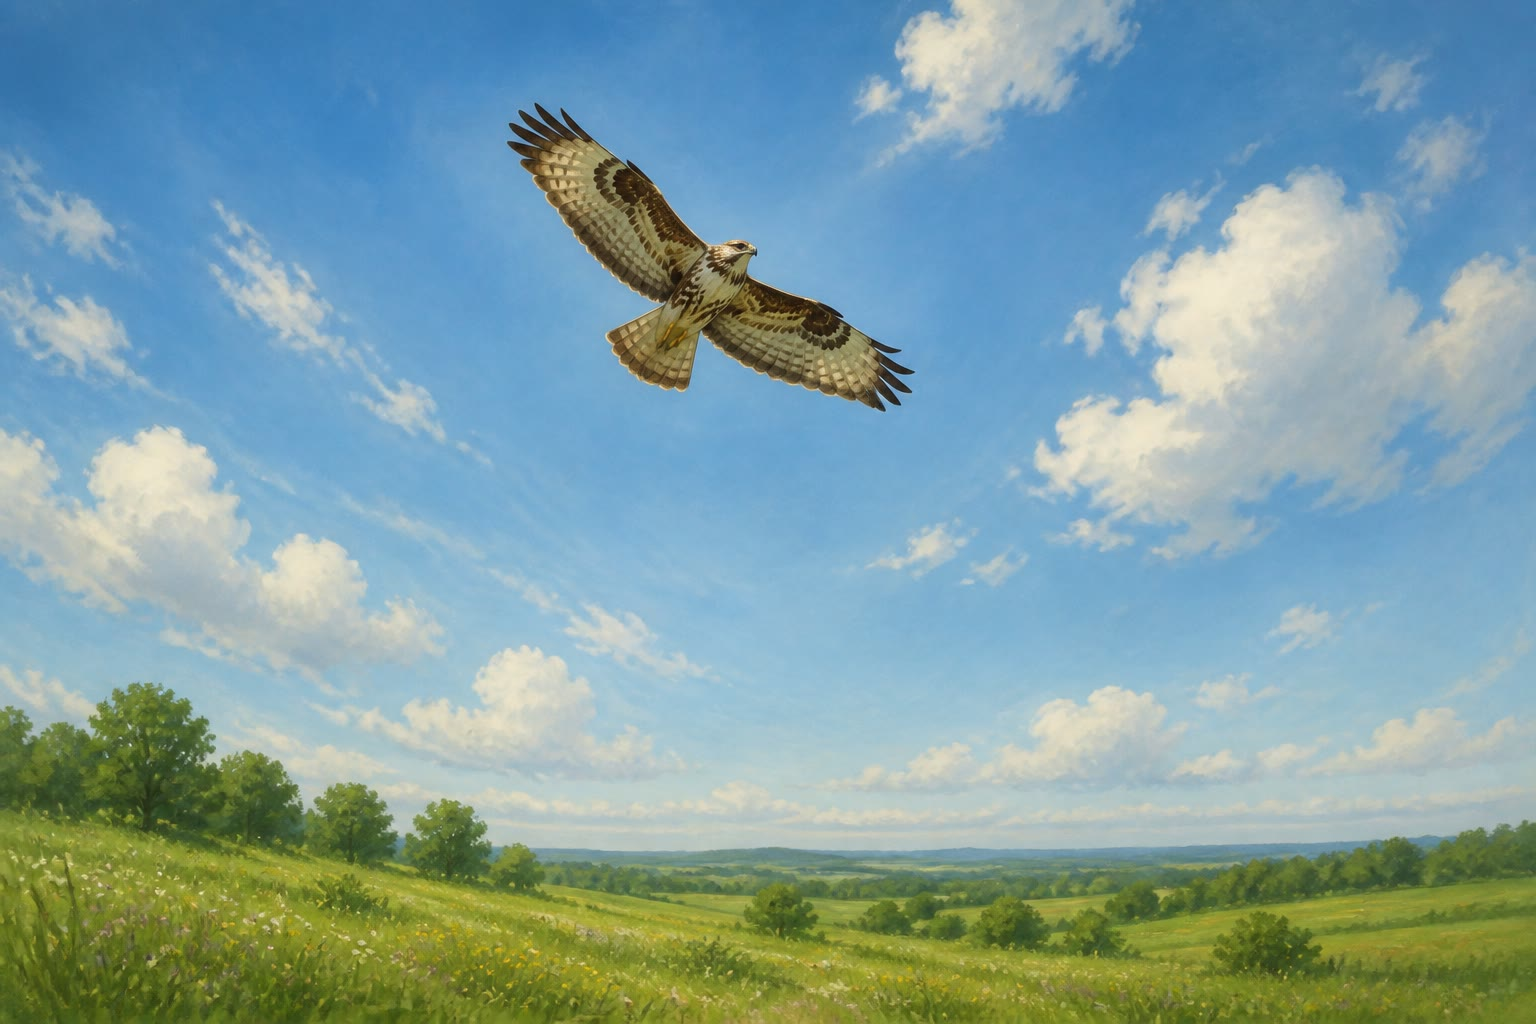
\includegraphics[width=0.6\linewidth]{images/book1/ai/g3-chains-buzzard.jpg}

{\small 草地\omterm{def:g3:food-chains:chain}{食物链}的最后一环正在巡逻：秃鹫的
下午，竟取决于往下数三个环节的草
长得有多绿。}
\end{omfigure}

\begin{method}[构建食物链]\label{met:g3:food-chains:build}
\begin{enumerate}
  \item 选择一种\omterm{def:g1:animals-around-us:animal}{动物}，问一问：它吃什么？把
        食物写在它的左边，箭头指向吃它的\omterm{def:g1:living-or-not:living}{生物}；
  \item 对这种食物问同样的问题，并继续向左
        直到找到\omterm{def:g1:plants-around-us:plant}{植物}；
  \item 再问：谁吃我选定的\omterm{def:g1:animals-around-us:animal}{动物}？只要
        还有吃它的\omterm{def:g1:living-or-not:living}{生物}，就继续向右延伸；
  \item 检查每个箭头都读作\omterm{def:g3:food-chains:chain}{“被……吃”}——食物
        沿箭头方向向右流动。
\end{enumerate}
\end{method}

\section{某个环节发生变化时}

\begin{proposition}[环节之间相互依赖]\label{prop:g3:food-chains:depend}
在\omterm{def:g3:food-chains:chain}{食物链}中，每个环节都依赖于它之前的环节，
并为它之后的环节提供食物。若某个环节变得稀少，
其后的环节就会缺食——而它\emph{之前}的环节，
因不再被大量吃掉，可能会增多。一个环节的
变化会沿着整条\omterm{def:g3:food-chains:chain}{食物链}传递。
\end{proposition}
\admitted

\begin{example}[干旱的夏天]\label{ex:g3:food-chains:dry}
干旱使草地的草变黄。蚱蜢缺少食物，
数量很少；以它们为食的蜥蜴也会挨饿，
进而很难为秃鹫提供食物。一个变黄的第一
环节，使上方的整条链条都变得稀薄——秃鹫从未吃过草，
却也感受到了干旱。
\end{example}

\begin{example}[移除捕食者]\label{ex:g3:food-chains:hunter}
假设山谷中的秃鹫消失了。蜥蜴
被捕食得少，数量增多；蚱蜢
则被吃得更厉害而减少；草因少被啃食，甚至可能更茂密。
移除\emph{最后}一个环节，影响同样会沿\omterm{def:g3:food-chains:chain}{食物链}向下传递——
只是方向相反。
\end{example}

\begin{remark}[真实的草地是食物网]\label{rem:g3:food-chains:web}
我们的链条只是一根线，但秃鹫也吃老鼠，
蜥蜴也吃苍蝇，草也是兔子的食物。
许多链条交错，便织成一张网——正是\emph{食物网}，
留待以后年级研究的内容。
（在\cref{ch:g2:what-animals-eat}中已经以狐狸、兔子和草
来暗示过这一点）。先学链条：它们是
编织这张网的线。
\end{remark}

\section{练习}

\begin{exercise}[$\star$]\label{exo:g3:food-chains:1}
\omterm{def:g3:food-chains:chain}{食物链}中的箭头表示什么？
它指向哪个方向？
\end{exercise}

\begin{exercise}[$\star$]\label{exo:g3:food-chains:2}
什么样的\omterm{def:g1:living-or-not:living}{生物}总是第一个环节？为什么？
\end{exercise}

\begin{exercise}[$\star$]\label{exo:g3:food-chains:3}
写出本章的草地\omterm{def:g3:food-chains:chain}{食物链}，包括它的四个环节和
箭头。
\end{exercise}

\begin{exercise}[$\star$]\label{exo:g3:food-chains:4}
改正这条\omterm{def:g3:food-chains:chain}{食物链}：狐狸 $\rightarrow$ 兔子 $\rightarrow$
草。
\end{exercise}

\begin{exercise}[$\star$]\label{exo:g3:food-chains:5}
用这些环节组成一条\omterm{def:g3:food-chains:chain}{食物链}：蓝山雀、橡树叶、
雀鹰、\omterm{ex:g2:animals-grow-up:butterfly}{毛毛虫}。
\end{exercise}

\begin{exercise}[$\star$]\label{exo:g3:food-chains:6}
在花园\omterm{def:g3:food-chains:chain}{食物链}生菜 $\rightarrow$ 蜗牛 $\rightarrow$
刺猬中，谁被蜗牛吃？谁吃蜗牛？
\end{exercise}

\begin{exercise}[$\star$]\label{exo:g3:food-chains:7}
利用\cref{met:g3:food-chains:build}，组成一条至少
三个环节的\omterm{def:g3:food-chains:chain}{食物链}，并以池塘里的苍鹭结尾。
\end{exercise}

\begin{exercise}[$\star$]\label{exo:g3:food-chains:8}
在\cref{ex:g3:food-chains:dry}的干燥夏天里，
秃鹰虽然从不吃草，为什么仍会受苦？
\end{exercise}

\begin{exercise}[$\star\star$]\label{exo:g3:food-chains:9}
有些园丁把每只蜗牛都毒死，结果有时会失去刺猬，
——然后反而遇到比以前\emph{更多}的蛞蝓和蜗牛。
用
\cref{prop:g3:food-chains:depend}解释这两方面的原因。
\end{exercise}

\begin{exercise}[$\star\star$]\label{exo:g3:food-chains:10}
“蜥蜴依赖于草。”这句话对还是错？
用草地\omterm{def:g3:food-chains:chain}{食物链}为你的答案辩护，并说明
草的减少会沿哪个方向传递。
\end{exercise}
